

%!TEX root = ../Notes.tex
\section{Connectedness} 
\subsection{Connected Sets and Spaces} 
\begin{definition}
	$(X,F_X)$ is a topological space. Then $X$ is \textbf{disconnected} if $X$ has a proper, nonempty, clopen subset. Otherwise, $X$ is \textbf{connected}.
	
	Equivalently, $X$ is disconnected if there exist nonempty, disjoint $A,B \in F_X$ such that $A \cup B = X$. $A$ and $B$ are called a separation of $X$. 
\end{definition}

Recall from Math 131 that $A \subseteq \R$ is connected iff $A$ is an interval. 
\begin{theorem}
	Let $f : (X,F_X) \to (Y,F_Y)$ be continuous. Then $X$ is connected only if $f(X)$ is connected. 
\end{theorem}
\begin{proof}
	Suppose that $U,V \in F_Y$ are separating sets of $f(X)$. Then, as $f$ is continuous, $f^{-1}(U)$ and $f^{-1}(V)$ are open. As $U$ and $V$ cover $f(X)$, $f^{-1}(U)$ and $f^{-1}(V)$ cover $X$. Furthermore, suppose that $x \in f^{-1}(U) \cap f^{-1}(V)$. Then $f(x) \in U \cap V$, and $f(x) \in f(X)$. However, this contradicts the assumption that $U$ and $V$ are separating sets. So $f^{-1}(U)$ and $f^{-1}(V)$ are disjoint open sets that cover $X$, so they are a separating set. But $X$ is connected, so this is a contradiction. Hence, no such $U$ and $V$ exist, and $f(X)$ is also connected. 
\end{proof}

Are the following connected? 
\begin{itemize}
	\item $\R$ with the finite complement topology - Yes. Let $U$ be some proper, nonempty open subset of $\R$. Then it is infinite, so its complement does not have finite complement. Therefore, its complement is not open. So there are no proper, nonempty clopen sets, and the topology is connected. 
	\item $\R$ with the half-open interval topology - No. Let $U = [0,\infty)$ and $V = (-\infty,0)$. These are open as $U = \bigcup_{n\in \N} [0,n)$ and $V = \bigcup_{n \in \N} [-n,0)$, and the arbitrary union of basis elements is open. Furthermore, they are clearly disjoint, and cover $\R$. 
\end{itemize}

We can also define (dis)connectedness for subsets of a topological space. 
\begin{definition}
	$(X,F_X)$ is a topological space. $S \subseteq X$ is \textbf{disconnected} if and only if there exist $U,V \in F_X$ such that $(U \cap S) \cap (V \cap S) = \emptyset$, $U \cap S, V \cap S \neq \emptyset$ and $S \subseteq U \cup V$. Note that this does not require $U \cap V = \emptyset$. 
\end{definition}
\begin{smallfact}
	$(X, F_X)$ is connected if and only if $\forall \ f : X \to Y$ where $Y$ has the discrete topology and $f$ is continuous, then $f$ constant. 
\end{smallfact}
\begin{proof}
	\begin{itemize}
		\item[$(\Rightarrow)$] Suppose $(X,F_x)$ is connected and that $\exists \ f : X \to Y$ where $Y$ has the discrete topology, such that $f$ is continuous and not constant. So there exist $p,q \in Y$ such that $p \neq q$ and $f^{-1}(\{p\}), f^{-1}(\{q\}) \neq \emptyset$. Therefore, $U = f^{-1}(\{p\})$ and $V = f^{-1}(\{p\}^c) \supseteq f^{-1}(\{q\})$ have $U,V \neq \emptyset$. As every set is open in the discrete topology and $f$ is continuous, $U,V \in F_X$. Furthermore, as $\{p\} \cap \{p\}^c = \emptyset$, $U \cap V = \emptyset$, and $U \cup V = f^{-1}(Y) = X$. So $U$ and $V$ separate $X$. However, $X$ is connected, so this is a contradiction, and no such $f$ exists. 
		\item[$(\Leftarrow)$] Suppose that $f : X \to Y$ is constant for all continuous $f$ where $Y$ has the discrete topology and that $X$ is disconnected. Then there exist separating sets $A,B \in F_X$. Define $Y = \{0,1\}$ with the discrete topology and $f : X \to Y$ as
		\[f(x) = \left\{ 
		\begin{array}{cc}
			0 & x \in A \\
			1 & x \in B 
		\end{array}
		\right.\]
		Then, as $f^{-1}(\{0\}) = A \in F_X$, $f^{-1}(\{1\}) = B \in F_X$, $f^{-1}(\emptyset) = \emptyset \in F_X$ and $f^{-1}(Y) = X \in F_X$, $f^{-1}(U) \in F_X$ for all $U \subseteq Y$ such that $U$ is open. So $f$ is continuous. Furthermore, as $A,B \neq \emptyset$, there exist $a \in A$ and $b \in B$, so $f(a) = 0$ and $f(b) = 1$. Hence $f$ is not constant. Therefore $f : X \to Y$ is a continuous function from $X$ to a space with the discrete topology that is not constant. This contradicts the initial assumption, so $X$ is connected. 
	\end{itemize}
\end{proof}

We now have an Important Lemma about Flowers. 
\begin{lemma}
	Suppose \{$y_j \mid j \in J$\} is a collection of connected subspaces of $X = \displaystyle{\bigcup_{j \in J} y_j}$, and $\displaystyle{\bigcap_{j \in J} y_j} \neq \emptyset$. Then $X$ is connected. 
\end{lemma}
\begin{proof}
	Suppose that $X$ is \textit{dis}connected. Then $X$ has a separation, $U, V$.
	\[ 
	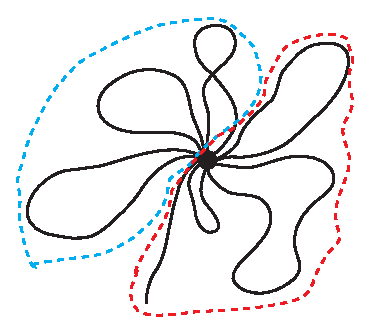
\includegraphics[width=200pt]{images/connectedness/flower} \]
	
	Let $j_0 \in J$. We know that 
	\begin{itemize}
		\item $(U\cap y_{j_0}) \cup (V\cap y_{j_0}) = y_{j_0}$, 
		\item $(U\cap y_{j_0}) \cap (V\cap y_{j_0}) = \emptyset$, 
		\item $(U\cap y_{j_0})$ and $(V\cap y_{j_0})$ are open in $y_{j_0}$, 
		\item $y_{j_0}$ is connected, so either $U \cap y_{j_0} = \emptyset$ or $V \cap y_{j_0} = \emptyset$. 
	\end{itemize}
	Without loss of generality, say $U \cap y_{j_0} = \emptyset$. Then $V \cap y_{j_0} = y_{j_0}$. By the same argument, $\forall j\in J, y_j \subseteq U$ or $y_j \subseteq V$.
	
	But $\displaystyle{\bigcap_{j \in J} y_j} \neq \emptyset$, so there exists $p\in \displaystyle{\bigcap_{j \in J} y_j}$ such that $p\in y_{j_0} \subseteq V$. Thus $\forall j\in J$, $y_j \subseteq V$.
	
	Since $X = \displaystyle{\bigcup_{j \in J} y_j} \subseteq V$, $U, V$ is not a separation of $X$. Thus, $X$ is connected. 
\end{proof}
\begin{theorem}
	Let $(X, F_X)$ and $(Y, F_Y)$ be topological spaces. Then $(X\times Y, F_{X\times Y})$ is connected if and only if both $X$ and $Y$ are connected. 
\end{theorem}
\begin{proof}
	\begin{itemize}
		\item[$(\Rightarrow)$] $\pi_X: X\times Y \longrightarrow X$ and $\pi_Y: X\times Y \longrightarrow Y$ are continuous surjections. Continuous functions preserve connectedness, so $X$ and $Y$ are connected. 
		\item[$(\Leftarrow)$] First, a picture proof.
		\[ 
		
\includegraphics[width=0.9 
		\textwidth]{images/connectedness/XxYconnected_comic}\]
		The axes are connected, because $X$ and $Y$ are connected. If we make a copy of the axes, shifted over a little bit, that copy is connected too. The union of these shifted axis crosses will be the entirety of $X\times Y$, and their intersection will be nonempty, so $X\times Y$ is connected.
		
		Now for the actual proof. Let $(x_0, y_0) \in X\times Y.$ Since $\{x_0\}\times Y \cong Y$, it is connected (as connectedness is a top. prop.). Similarly, $\{y_0\} \times X$ is connected.
		
		Observe that $(x_0, y_0) \in (\{x_0\}\times Y) \cap (\{y_0\} \times X)$. That is, $(\{x_0\}\times Y) \cap (\{y_0\} \times X) \neq \emptyset$. Then $(x_0, y_0) \in (\{x_0\}\times Y) \cup (\{y_0\} \times X)$ is connected by the Important Flower Lemma. By the same process, we see that $\forall x\in X$, $(X\times \{y_0\}) \cup (\{x\} \times Y)$ is connected.
		
		Note that $(X\times \{y_0\}) \subseteq \displaystyle{\bigcap_{x \in X}(X\times \{y_0\}) \cup (\{x\} \times Y)}$.
		
		\textbf{Claim:} $\displaystyle{\bigcup_{x \in X}(X\times \{y_0\}) \cup (\{x\} \times Y)} = X\times Y$. 
		
		\textbf{Proof of claim:} 
		\begin{itemize}
			
			\item[$(\subseteq)$] Clearly $\displaystyle{\bigcup_{x \in X}(X\times \{y_0\}) \cup (\{x\} \times Y)} \subseteq X\times Y$ because $X\times Y$ is the entire space. 
			
			\item[$(\supseteq)$] Let $(x_1, y_1) \in X\times Y$. Then $(x_1, y_1) \in (\{x_1\}\times Y)$. Thus, $\forall x\in X$ and $y\in Y$, $(x,y) \in (\{x\} \times Y) \subseteq {\displaystyle\bigcup_{x \in X}(X\times \{y_0\}) \cup (\{x\} \times Y)}$. 
		\end{itemize}
		
		Since $(X\times \{y_0\}) \cup (\{x\} \times Y)$ is connected $\forall x\in X$, and $\displaystyle{\bigcap_{x \in X}(X\times \{y_0\}) \cup (\{x\} \times Y)}\neq \emptyset$, $X\times Y$ is connected by the Important Flower Lemma. 
	\end{itemize}
\end{proof}

\subsection{Connected Components} 
\begin{definition}
	Let $(X, F_X)$ be a topological space and let $p\in X$. Let $\{C_j\mid j\in J\}$ be the set of all connected subspaces of $X$ containing $p$. Then ${\cup_{j\in J}C_j}$ is said to be the \textbf{connected component}, $C_p$, of $p$. 
\end{definition}

And now, a series of tiny facts about connected components. 
\begin{smallfact}
	Let $(X, F_X)$ be a topological space. Then, 
	\begin{enumerate}
		\item $\forall p \in X$, $C_p$ is connected. 
		\item If $C_p$ and $C_q$ are connected components, then either $C_p\cap C_q = \emptyset$ or $C_p = C_q$. (That is, connected components partition a space.) 
	\end{enumerate}
\begin {proof} 
\begin{enumerate}
	\item $p\in {\cap_{j\in J} C_j}$, so $C_p = {\cup_{j\in J} C_j}$ is connected by the lemma above. 
	\item Suppose $C_p \cap C_q \neq \emptyset$ and let $x\in C_p \cap C_q$. Then $C_p \cup C_q$ is connected by the lemma above.
	
	$p\in C_p \cup C_q$, so $C_p \cup C_q \in \{C_j\mid j\in J\}$. Also, $C_p \cup C_q \subseteq C_p$, since $C_p = {\cup_{j\in J} C_j}$. So, $C_q \subseteq C_p$. Similarly, $C_p \subseteq C_q$. 
\end{enumerate}
Thus $C_p = C_q$, so we can say $X$ is partitioned by its connected components. 
\end{proof}
\end{smallfact}
\begin{example}
Let $X = \R^2$ with the dictionary topology. Connected components are vertical lines. (Proof is an exercise.) Define $x\sim y$ ($x, y \in \R^2$) if $x$ and $y$ are in the same connected component. Then $X/\sim$ = $\R$ with the discrete topology. 

\[ 
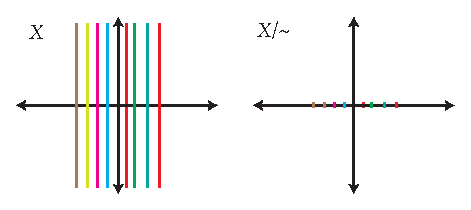
\includegraphics[width=300pt]{images/connectedness/dictionary_sim}\]
\end{example}

Connectedness is not always intuitive, though. Here's a large example showing this.

Define the Comb, the Flea, and the space $X$ as follows. 
\begin{itemize}
\item[Comb:] ${\displaystyle\bigcup_{n=0}^{\infty}y_n}$ in $\R^2$ where $y_0 = [0,1]\times\{0\}$ and $\forall n\in \N$, $y_n = \{1/n\} \times [0,1]$. 
\item[Flea:] $\{(0,1)\}$. 
\item[$X$:] Flea $\cup$ Comb with the subspace topology. 
\end{itemize}
\begin{example}
$X$ is connected. 
\end{example}
\begin{proof}
First, we claim that the Comb is connected. 

Proof: 

$\forall n \in \{0\} \cup \N$, $y_n$ is connected because $y_n \cong [0,1]$. Also, $\forall n \in \N$, $y_0 \cap y_n \neq \emptyset$ (because $(1/n, 0)$ is in both), so $y_0 \cup y_n$ is connected. 

Thus ${\displaystyle\bigcap_{n\in \N}y_0 \cup y_n} \neq \emptyset$, so ${\displaystyle\bigcup_{n=0}^{\infty}y_0 \cup y_n} = {\displaystyle\bigcup_{n=0}^{\infty}y_n} $ and so the Comb is connected by the Important Flower Lemma. 
\begin{flushright}
$\Box$ 
\end{flushright}

Now we want to show that $X$ is connected. Suppose $U$, $V$ are a separation of $X$. Since the Comb is connected, we can say, WLOG, that Comb $\subseteq U$. Then it must be that Flea $\subseteq V$ because $U$, $V$ are a separation. $V$ is open in $X$, so $\exists \epsilon > 0$ s.t. $B_{\epsilon}((0,1); X) \subseteq V$. Let $n \in \N$ s.t. $n > \frac{1}{\epsilon}$. Then $d((\frac{1}{n}, 1), (0, 1)) = \frac{1}{n} < \epsilon \Rightarrow (1/n, 1) \in B_{\epsilon}((0,1); X) \subseteq V$. Observe that since $Y_n = \{1/n\} \times [0,1]$, $(1/n, 1) \in Y_n$. Thus, $(1/n, 1) \in V \cap Y_n \subseteq V \cap Y \subseteq V \cap U \Rightarrow V \cap U \neq \emptyset$. But this is a contradiction, since we assumed that $U$, $V$ was a separation of $X$. Thus, $X$ is connected. 
\end{proof}

\section{Path-Connectedness} 
\begin{definition}
Let $(X, F_X)$ be a topological space and let $f:[0,1] \rightarrow X$ be continuous. Then we say that $f$ is a \textbf{path} from $f(0)$ to $f(1)$ (Note: it is handy to think of $t \in [0,1]$ as time). 
\end{definition}
\begin{definition}
Let $(X, F_X)$ be a topological space. If $\forall p$, $q \in X$, there exists a path in $X$ from $p$ to $q$ then we say that $X$ is \textbf{path-connected}. 
\end{definition}
\begin{example}
$\R^n$ is path-connected:

Let $a$, $b \in \R^n$ be given. Let $f: I \rightarrow \R^n$ be $f(t) = (1-t)a + bt$. Then $f(0) = a$, and $f(1) = b$. $f$ can be shown to be continuous by performing an involved $\epsilon$-$\delta$ proof. 
\end{example}

Some remarks: 
\begin{enumerate}
\item Connected is a negative definition and path-connected is a positive definition (for connectedness, we are trying to show that a separation \emph{doesn't} exist, so it is easiest to do connectedness proofs by contradiction. For path-connectedness, we are trying to show that a path exists, so path-connectedness proofs are more easily done constructively). 
\item In general, it is easier to prove that a space is disconnected than to prove that it is not path-connected. 
\item In general, it is easier to prove that a space is path-connected than to prove that it is connected. 
\end{enumerate}
\begin{theorem}
If $(X, F_X)$ is path-connected, then $(X, F_X)$ is connected. 
\end{theorem}
\begin{proof}
Suppose there exists a separation $U$, $V$ of $X$. Since $U$, $V$ is a separation of $X$, $U \neq \emptyset$, $V \neq \emptyset$. Let $p \in U$, $q \in V$ be given. Since $X$ is path-connected, $\exists$ a path $f$ from $p$ to $q$. Since paths are continuous by definition, $f$ is continuous, so $f^{-1}(U)$, $f^{-1}(V)$ are open in $[0,1]$. 

\emph{Claim 1:} $f^{-1}(U) \cup f^{-1}(V) = [0,1]$. \\
\emph{Proof of Claim 1:} Let $x \in [0,1]$ be given. Then $f(x) \in X = U \cup V \Rightarrow f(x) \in U$ or $f(x) \in V \Rightarrow x \in f^{-1}(U)$ or $x \in f^{-1}(V) \Rightarrow x \in f^{-1}(U) \cup f^{-1}(V)$. Thus, $[0,1] \subseteq f^{-1}(U) \cup f^{-1}(V) \Rightarrow [0,1] = f^{-1}(U) \cup f^{-1}(V)$ (since $f^{-1}(U)$, $f^{-1}(V) \subseteq [0,1]$).

\emph{Claim 2:} $f^{-1}(U) \cap f^{-1}(V) = \emptyset$. \\
\emph{proof of Claim 2:} Suppose $\exists x \in f^{-1}(U) \cap f^{-1}(V)$. Then $x \in f^{-1}(U) \Rightarrow f(x) \in U$, and $x \in f^{-1}(V) \Rightarrow f(x) \in V$, so $f(x) \in U \cap V$, which is impossible since we are assuming that $U$ and $V$ are a separation of $X$. Thus, $f^{-1}(U) \cap f^{-1}(V) = \emptyset$.

Observe that since $f$ is a path from $p$ to $q$, $f(0) = p$ and $f(1) = q$, so $0 \in f^{-1}(U)$, $1 \in f^{-1}(V)$ so $f^{-1}(U)$ and $f^{-1}(V)$ are non-empty and proper. Thus, since $f^{-1}(U) \cap f^{-1}(V) = \emptyset$ and $f^{-1}(U) \cup f^{-1}(V) = [0,1]$, $f^{-1}(U)$ and $f^{-1}(V)$ form a separation of $[0,1]$. But this is a contradiction, since we know from Math 131 that $[0,1]$ is connected. Thus, $(X, F_X)$ must be connected. 
\end{proof}

Recall the example of the flea and the comb. We showed that the flea and comb is connected. 
\begin{theorem}
The flea and comb is not path-connected. 
\end{theorem}
\begin{proof}
We want to show that $\nexists$ a path from the flea to $(0,0)$. 

Suppose $\exists$ a path $f$ from the flea to $(0,0)$. Let $p =$ flea. Then $f^{-1}(\{p\})$ is not empty because $f(0) = p$ by the definition of $f$. Similarly, by the definition of $f$, $f(1) = (0,0) \neq p$, so $f^{-1}(\{p\})$ is proper as well. Observe that since $\{p\}$ is closed in $X$ and $f$ is continuous, $f^{-1}(\{p\})$ is closed.

We'd like to show that $f^{-1}(\{p\})$ is open, since then it would be a nontrivial clopen subset of the flea and the comb. This implies that the set is not connected, a contradiction.

Let $y \in f^{-1}(\{p\})$ be given. 

Observe that $B_{\frac{1}{2}}(p; X)$ is open in $X$. Since $f$ is a path, $f$ is continuous, so $f^{-1}(B_{\frac{1}{2}}(p; X))$ is open in $[0,1]$. Since $y \in f^{-1}(\{p\})$, $f(y) = p \in B_{\frac{1}{2}}(p; X) \Rightarrow y \in f^{-1}(B_{\frac{1}{2}}(p; X))$. Thus, since $f^{-1}(B_{\frac{1}{2}}(p; X))$ is open in $[0,1]$, $\exists \epsilon > 0$ s.t. $B_{\epsilon}(y; [0,1]) \subseteq f^{-1}(B_{\frac{1}{2}}(p; X))$.

Let $z \in B_{\epsilon}(y; [0,1])$. If $f(z) = p$, then $B_{\epsilon}(y; [0,1]) \subseteq f^{-1}(p)$ and so $f^{-1}(p)$ is open, completing the proof.

Suppose $f(z) \neq p$. Since $z \in B_{\epsilon}(y; [0,1])$, $z \in f^{-1}(B_{\frac{1}{2}}(p; X))$, so $f(z) \in B_{\frac{1}{2}}(p; X)$ (so $d(f(z), p) < \frac{1}{2}$). Since $Y_0 = [0,1] \times \{0\}$, for each $q \in Y_0$, $d(p,q) \geq 1 \Rightarrow q \not\in B_{\frac{1}{2}}(p; X)$. Thus, $f(z) \not\in Y_0$. Thus since $f(z) \neq p$, $\exists n \in \N$ s.t. $f(z) \in Y_n$.

There exists $r\in \R\setminus\Q$ such that $0 < r < \frac{1}{n}$. Define sets $A, B\subseteq f\left( B_{\epsilon} (y;[0,1]) \right)$, as
\[A = \left\{ (x,y)\in f\left( B_{\epsilon} (y;[0,1]) \right) | x< r\right\} \hspace{.15in} \text{and} \hspace{.15in} B = \left\{ (x,y)\in f\left( B_{\epsilon} (y;[0,1]) \right) | x> r\right\}\]
We next show that $A$ and $B$ are a separation for $f\left( B_{\epsilon} (y;[0,1]) \right)$. To this end, we'll need to show that $A$ and $B$ are disjoint, proper and non-empty, that their union is the entire set, and that they're are both clopen.

We note that $A\cap B = \emptyset$ by definition. We know that $f(z)\in B$, and $p\in A$, so neither set will be empty and both will be proper.

Next, we want to show that $A\cup B = f\left( B_\epsilon (y;[0,1]) \right)$. Certainly $A\cup B \subseteq f\left( B_{\epsilon} (y;[0,1]) \right)$. Now let $(x, f(x)) \in f\left( B_{\epsilon} (y;[0,1]) \right)$. We know that $f(x) \neq 0$, and in fact $x = \frac{1}{m}$ for some $m\in \N$. Then $x\neq r$, so $x\in A\cup B$ and we're done.

Next we want to show that $A$ is open in $f(B_{\epsilon} (y;[0,1]))$. We know that $\{(x,y) | x<r \}$ is open in $\R^2$, the half plane to the left of $r$. It follows using the subspace topology that $A = \{ (x,y) | x< r \} \cap f\left( B_{\epsilon} (y;[0,1]) \right)$ is open in $f\left( B_{\epsilon} (y;[0,1] ) \right)$. Similarly, $B$ is open in $f\left( B_{\epsilon} (y;[0,1] ) \right)$. Since each is the other's complement in $f\left( B_{\epsilon} (y;[0,1] ) \right)$, then both are also closed.

We've hence shown that $A$ and $B$ are a separation of $f\left( B_{\epsilon} (y;[0,1] ) \right)$. This is a contradiction, since $B_{\epsilon} (y;[0,1])$ is connected and $f$ is continuous, and thus we've disconnected $B_{\epsilon}(y;[0,1])$. We conclude that $f(z) = p$, for all such $z\in B_{\epsilon}(y;[0,1])$. 

Therefore $B_{\epsilon} (y;[0,1]) \subseteq f^{-1}(\{ p\})$, so $f^{-1} (\{p\})$ is open. So $f^{-1}( \{ p \} )$ is a clopen, non-empty, proper subset of $[0,1]$. This is a contradiction, so we conclude that there does not exist a path in $X$ from $p$ to $(0,0)$ (or anywhere). 
\end{proof}

The point of the whole example is to show that path-connected is stronger than connected. We knew already that path-connected implies connected, and now we see that connected doesn't necessarily imply path-connected.

\subsection{Combining paths} It turns out that it's useful to have a way to combine paths. 
\begin{definition}
Let $f,g$ be paths in a topological space $(X,F_X)$ such that $f(1) = g(0)$. Then we define $f\ast g : I \to X$ by
\[ (f\ast g )(t) = 
\begin{cases}
f(2t) & 0 \leq t\leq \frac{1}{2} \\
g(2t-1) & \frac{1}{2} \leq t \leq 1 
\end{cases}
\]
\end{definition}

Intuitively what's happening is that we're connecting two paths while speeding things up, creating a new single path parametrized from 0 to 1 from two paths which were parametrized from 0 to 1. 
\begin{smallfact}
$f\ast g$ is a path from $f(0)$ to $g(1)$. 
\end{smallfact}
\begin{proof}
By the Pasting Lemma\footnote{HW3 \#1, which states that if we have two continuous functions with closed sets as domains, and they agree over the intersection of these domains, then the combined function is continuous}, since $[0,\frac{1}{2}]$ and $[\frac{1}{2},1]$ are closed subsets under $[0,1]$, and $f(2 (\frac{1}{2} )) = f(1) = g(0) = g(2 (\frac{1}{2}) - 1 )$, $f\ast g$ is continuous. So $f\ast g$ is a path. Since $(f\ast g)(0) = f(0)$ and $(f\ast g) (1) = g(1)$, then $f\ast g$ is a path from $f(0)$ to $f(1)$. 
\end{proof}

This definition also allows us to create an analogue to the flower lemma. 
\begin{theorem}
[Flower Lemma for Path-connected] Let $X = \cup_{i\in I} Y_i$ such that $\forall i\in I$, $Y_i$ is path-connected, and $\cap_{i\in I} Y_i \neq \emptyset$. Then $X$ is path-connected. 
\end{theorem}
\begin{proof}
Let $a,b\in X$. If $\exists n\in I$ such that $a,b\in Y_n$, then there exists a path from $a$ to $b$ in $Y_n\subseteq X$. So without loss of generality, suppose that $a\in Y_n, b\in Y_m$, and $m\neq n$. Let $x\in \cap_{i\in I} Y_i$. Then there exists a path $f$ from $a$ to $x$ in $Y_n$, and a path $g$ from $x$ to $b$ in $Y_m$. So $f\ast g$ is a path in $X$ from $a \to b$, and we're done. 
\end{proof}
\begin{corollary}
The product of path-connected spaces is path-connected. 
\end{corollary}
\begin{proof}
The proof is identical to the connected one; the key is the flower lemma. 
\end{proof}
\begin{definition}
Let $(X,F_X)$ be a topological space, and $p\in X$. Let $\{C_j | j\in J\}$ be the set of all path-connected subspaces of $X$ containing $p$. Then $\cup_{j\in J} C_j$ is said to be the \textbf{path-connected component} $C_p$. 
\end{definition}

Some tiny facts about path-connected components:

Let $(X,F_X)$ be a topological space. Then 
\begin{enumerate}
\item $\forall p\in X, C_p$ is path-connected 
\item If $C_p, C_q$ are path-connected components, then either $C_p \cap C_q = \emptyset$, or $C_p = C_q$. In other words, path-connected components partition the set. 
\end{enumerate}
We'll omit this proof, as it is identical to the one presented on connectedness. 
